\section{灵敏度与失效分析}

\subsection{校准、残差与聚类敏感性}

四级消融表明，D0 曲线主要影响无扰流线性度：
\begin{equation}
u_{\mathrm{nor},L}: 0.462931\%\longrightarrow 0.055310\%.
\end{equation}
加入该曲线后，MAE 由 $0.179991\%$ 增至 $0.260279\%$，$u_{\mathrm{nor},d}$ 未同步改善。无扰流校准能够修复正常工况的流量相关偏差，但结果依赖 D0 锚点的覆盖范围。

在线剖面特征进入 Ridge 后，MAE 为 $0.091290\%$，$u_{\mathrm{nor},d}=0.085595\%$，说明线性模型已能解释部分扰流附加偏差；此时 $u_{\mathrm{nor},L}=0.046127\%$、$u_{\mathrm{nor},r}=0.080151\%$，仍超过阈值。RBF-KRR 将 MAE 降至 $0.055176\%$，并得到 $u_{\mathrm{nor},L}=0.024645\%$、$u_{\mathrm{nor},r}=0.064035\%$、$u_{\mathrm{nor},d}=0.083017\%$。物理--稳定性双核 KRR 加入逐秒稳定性特征后，标签盲划分中的最坏组重复性仍未达标。核映射对平均误差和扰流漂移较为有效，而重复性更依赖局部样本覆盖。

扰流聚类采用 KMeans、Ward 和对角 GMM，并令 $K=2,\ldots,5$。最高 Silhouette 系数为 $0.377676$，出现在 $K=2$ 的 KMeans；一个簇主要对应 D3，其余扰流编号大量重叠，系统漂移型与重复性失稳型也没有形成清晰边界。聚类数变化没有改变这一判断，因此使用统一 RBF-KRR 的连续相似性补偿。

\subsection{整组留出、OOD 与失效诊断}

普通分层验证会在同一 $h$ 单元内同时保留训练窗口和验证窗口。为模拟新日期或新工况，压力测试把完整重复单元
\begin{equation}
h=(\mathrm{date},\mathrm{flow\ point},\mathrm{disturbance\ id}),
\end{equation}
移出训练集，并用 $SD_h$ 记录留出单元内部的误差波动。$SD_h$ 只用于失效诊断，不替代官方按 $g=(\mathrm{date},\mathrm{flow\ point})$ 计算的 $SD_g$ 与 $u_{\mathrm{nor},r}$。压力测试未能实现全部指标同时达标。

在紧凑物理标准化特征空间中，最近邻 OOD 距离定义为
\begin{equation}
d_{\mathrm{OOD}}(x_i)=\min_{j\in \mathcal{T}}
\left\|\boldsymbol z_i-\boldsymbol z_j\right\|_2,
\end{equation}
其中 $\mathcal{T}$ 为训练窗口集合。保留全部压力测试组时，MAE 与 OOD 距离的 Pearson 相关系数为 $0.910943$，Spearman 系数仅为 $0.078788$。极端组 \texttt{20260607-60-D0} 的 OOD 距离达到 $54.8812$；删除该点后，Pearson 系数变为 $-0.305248$。高线性相关主要由正常锚点完整缺失驱动，普通扰流组的误差不能只由 OOD 距离解释。

\begin{figure}[!htbp]
  \centering
  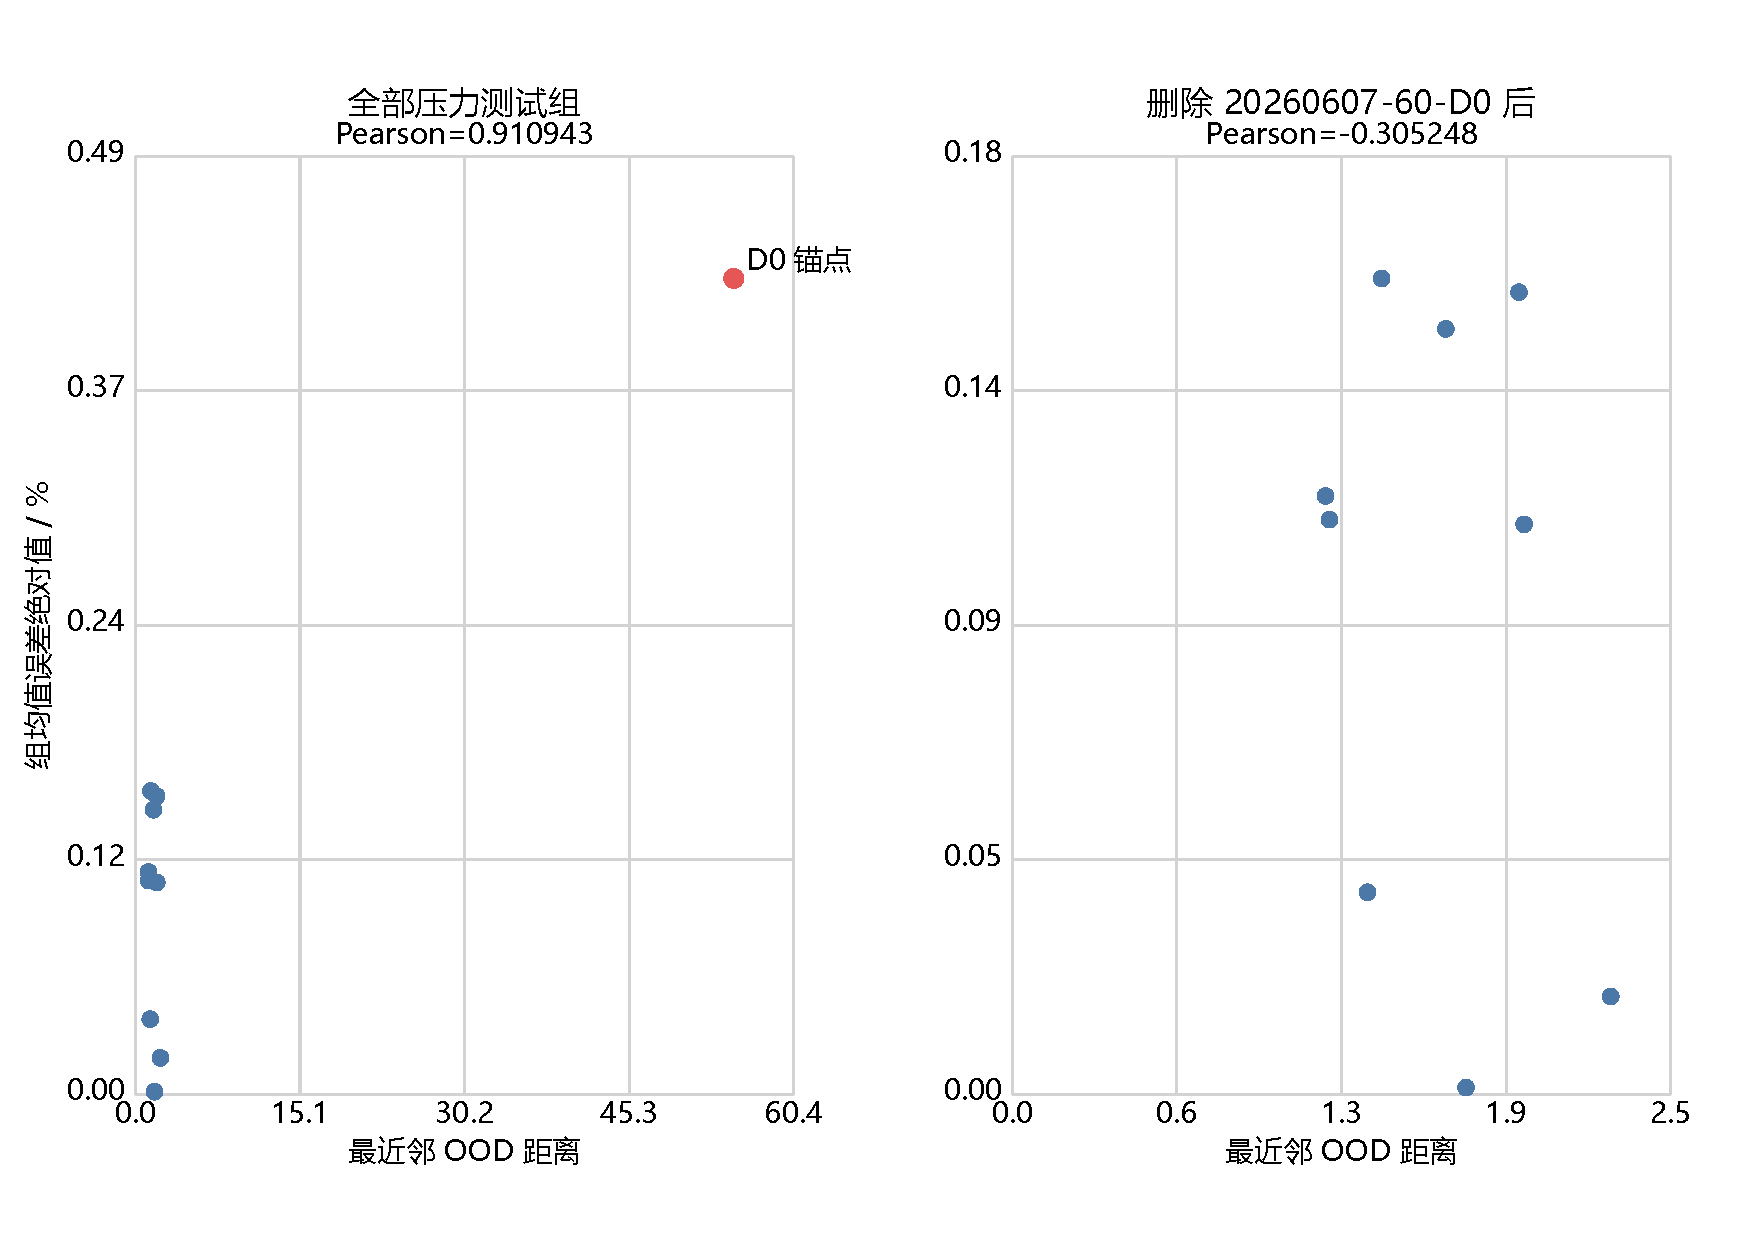
\includegraphics[width=0.92\textwidth]{../figures/fig_krr_ood_vs_error.pdf}
  \caption{压力测试全部组及删除极端 D0 锚点后的 OOD--误差关系}
  \label{fig:krr_ood}
\end{figure}

表~\ref{tab:failure_mechanisms} 将压力测试误差归纳为三类。正常锚点缺失表现为组内波动较小而均值偏差显著；扰流系统漂移表现为特定方向性扰流下的稳定偏差；重复性失稳则具有较小均值误差和较大的 $SD_h$，与窗口内短时剖面变化有关。

\begin{table}[!htbp]
\centering
\caption{整组留出压力测试的三类失效机制}
\label{tab:failure_mechanisms}
\scriptsize
\begin{tabular}{p{0.16\textwidth}p{0.22\textwidth}p{0.22\textwidth}p{0.26\textwidth}}
\toprule
失效类型 & 代表性工况 & 主要诊断量 & 机理解释 \\
\midrule
正常锚点缺失型 & \texttt{20260607-60-D0} & OOD 距离 $54.8812$，$|\bar e|=0.423406\%$，$SD=0.022659\%$ & 组内波动较小而均值偏差显著，属于正常标定锚点缺失引起的系统外推 \\
扰流系统漂移型 & \texttt{20260609-60-D5}；\texttt{20260613-60-D4} & $|\bar e|$ 分别为 $0.154697\%$、$0.115376\%$ & 特定方向性扰流产生稳定偏差，统一补偿函数仍有局部欠拟合 \\
扰流重复性失稳型 & \texttt{20260608-60-D7}；\texttt{20260615-60-D2} & 均值偏差相对较小，但单元内 $SD_h$ 超过 $0.040\%$ & 短时剖面或动态状态变化未被现有紧凑特征完全描述 \\
\bottomrule
\end{tabular}
\end{table}

图~\ref{fig:leave_one_group_heatmap} 给出逐组留出条件下扰流编号与流量点的平均误差，较大偏差集中在少数扰流与流量组合。

\begin{figure}[H]
  \centering
  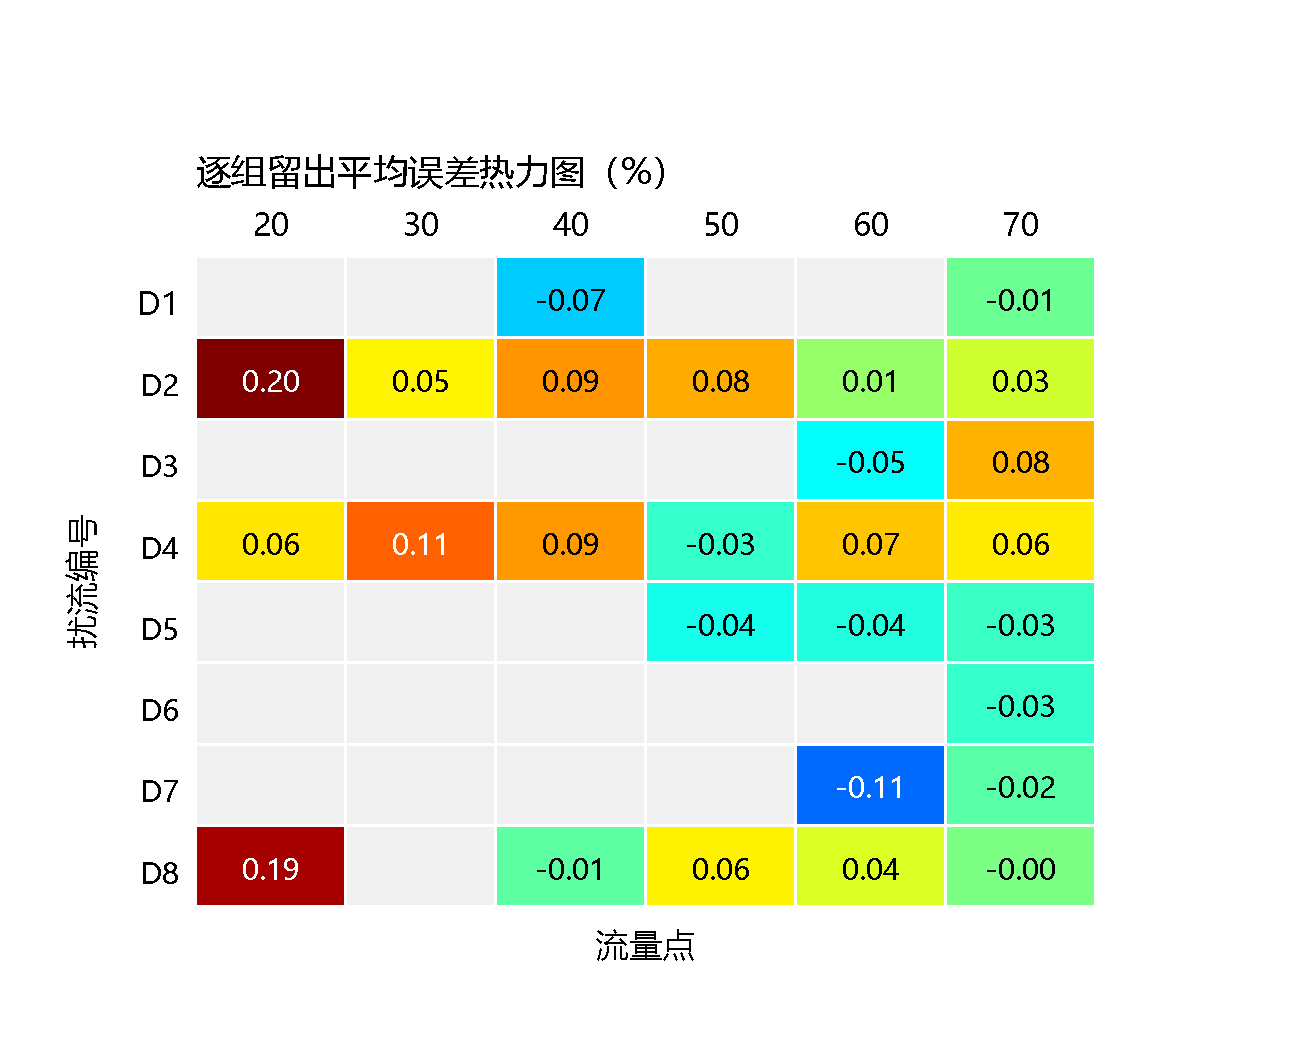
\includegraphics[width=0.78\textwidth]{../figures/fig_leave_one_group_error_heatmap.pdf}
  \caption{逐组留出平均误差热力图}
  \label{fig:leave_one_group_heatmap}
\end{figure}
